\documentclass{article}
\usepackage[T1]{fontenc}
\usepackage{lmodern}
\usepackage[polish]{babel}
\usepackage{graphicx}
\usepackage{float}
\usepackage{hyperref}
\usepackage{amsmath}
\usepackage{listings}
\usepackage{xcolor}

\usepackage[a4paper, margin=2.54cm]{geometry}

\title{Praca domowa 5\\Miary odległości}
\author{Damian Jankowski s188597}

\begin{document}

\maketitle

\section{Wstęp}

Celem pracy domowej było zapoznanie się z wybranymi miarami odległości.
Miary odległości odgrywają ważną rolę w uczeniu maszynowym. Są one
wykorzystywane do obliczania odległości między obserwacjami w celu
klasyfikacji nowych danych. W zależności od wybranej miary, wyniki
mogą się znacznie różnić. Dlatego też ważne jest, aby wybrać miarę
odpowiednią do danego problemu.

Dla przykładowych danych należało obliczyć odległości następującymi miarami:
\begin{itemize}
    \item miejska (Manhattan)
    \item euklidesowa
    \item Czebyszewa
\end{itemize}

Każda z tych miar jest rozszerzeniem tzw. odległości Minkowskiego, która jest
zdefiniowana następująco:

\begin{equation}
    L_m(x, y) = \left( \sum_{i=1}^{n} |x_i - y_i|^m \right)^{\frac{1}{m}}
\end{equation}
gdzie:
\begin{itemize}
    \item $x, y$ - wektory danych
    \item $n$ - liczba wymiarów
    \item $m$ - parametr miary
\end{itemize}

\subsection{Odległość miejska (Manhattan)}
Szczególny przypadek odległości Minkowskiego, dla $m=1$, wyrażona
wzorem:
\begin{equation}
    L_1(x, y) = \sum_{i=1}^{n} |x_i - y_i|
\end{equation}

Daje podobne wyniki jak odległość euklidesowa, ale odstające
wartości są stłumione przez brak podnoszenia ich do kwadratu.

\subsection{Odległość euklidesowa}
Jest to odległość Minkowskiego dla $m=2$, wyrażona wzorem:
\begin{equation}
    L_2(x, y) = \sqrt{\sum_{i=1}^{n} |x_i - y_i|^2}
\end{equation}

Najczęściej wykorzystywana miara odległości. Wadą tej miary jest
duża wrażliwość na wartości odstające z racji kwadratowego wykładnika.

\subsection{Odległość Czebyszewa}
Wyrażona wzorem:

\begin{equation}
    L_\infty(x, y) = \max_{i=1}^{n} |x_i - y_i| = \lim_{m \to \infty} L_m(x, y)
\end{equation}

Wprowadzona przez Pafnutija Czebyszewa. Jest to szczególny
przypadek odległości Minkowskiego, dla $m=\infty$. Wartość odległości
jest równa największej różnicy między wartościami wektorów.

W szachach odległość Czebyszewa jest równa liczbie ruchów króla, potrzebnych
do przejścia z jednego pola na drugie.

\section{Zadanie}

Do przećwiczenia wyznaczania tych miar wybrałem przykładowy zbiór danych:
\begin{equation}
    X = 
    \begin{bmatrix}
        -3.5 \\
        4.4 \\
        -2.2 \\
    \end{bmatrix} \quad
    Y =
    \begin{bmatrix}
        0.1 \\
        -2.5 \\
        3.9 \\
    \end{bmatrix}
\end{equation}

Obliczenia prezentuję poniżej:
\begin{figure}[H]
    \centering
    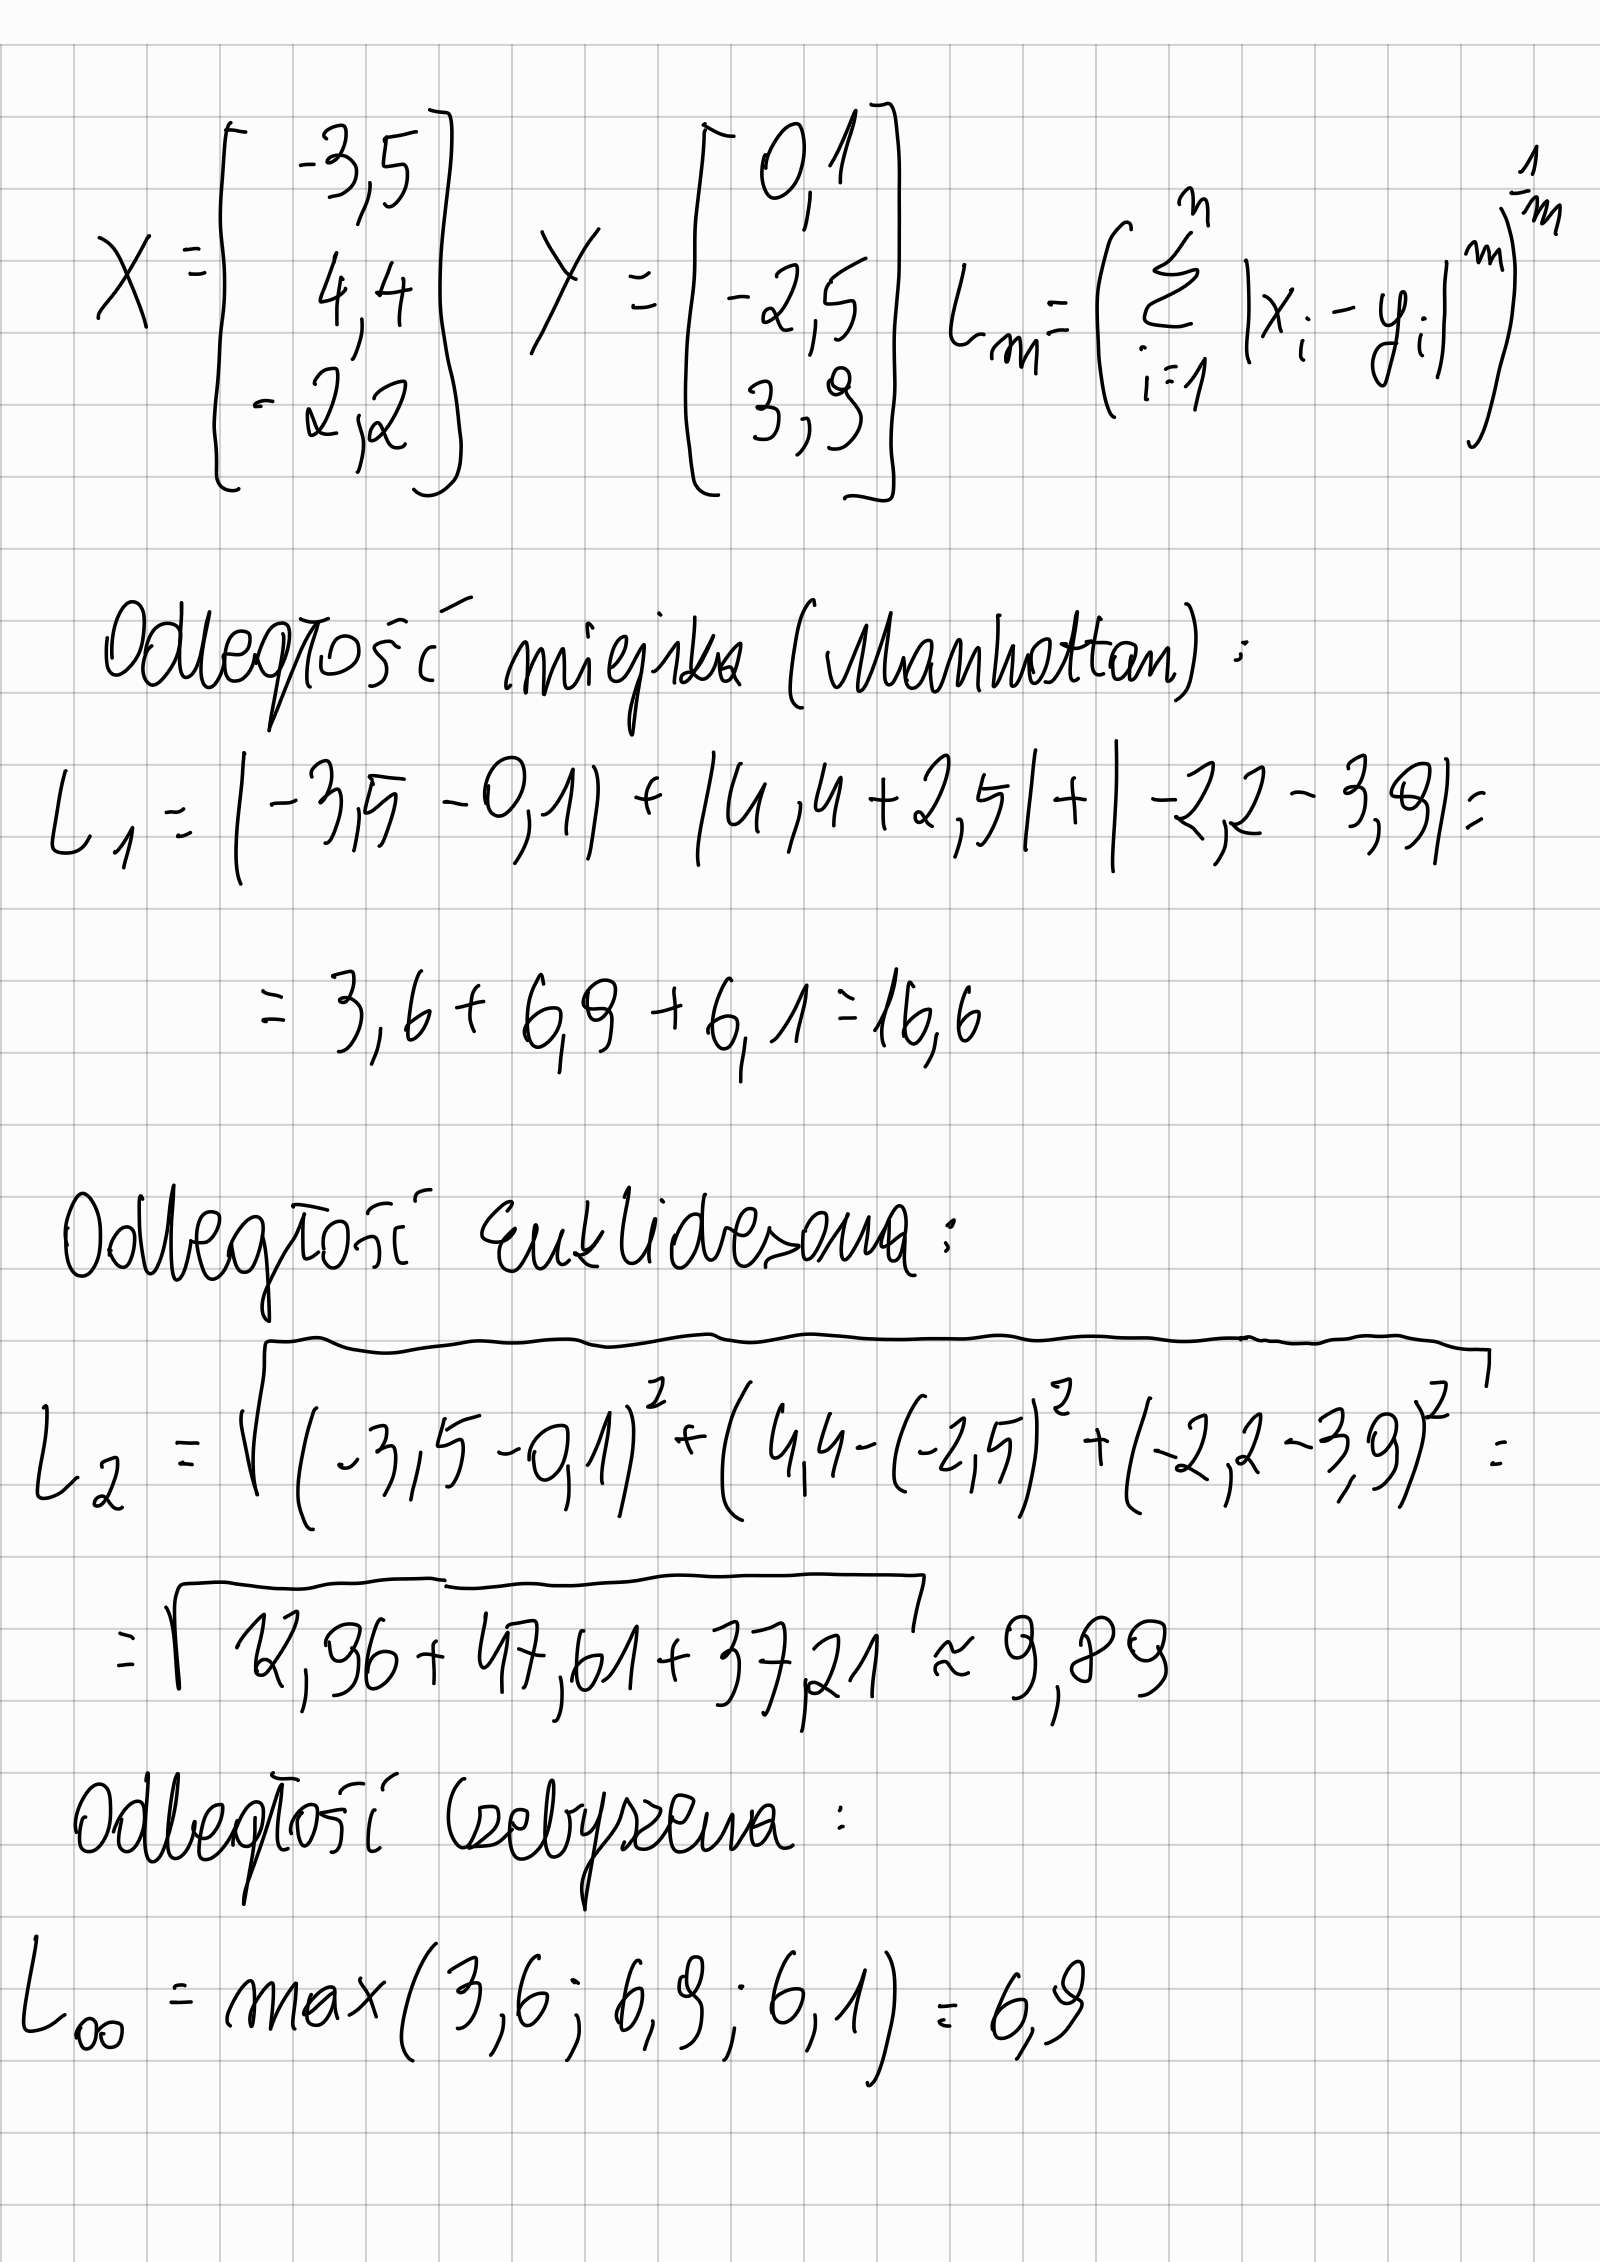
\includegraphics[width=0.7\textwidth]{rozwiazanie.jpg}
\end{figure}

By sprawdzić poprawność obliczeń napisałem krótki skrypt w języku Python:
\lstinputlisting[
language=python,  
basicstyle=\small\tt,
keywordstyle=\color{blue},
backgroundcolor=\color{cyan!10}
]{main.py}

Wynik działania programu:
\begin{lstlisting}[basicstyle=\small\tt,,
backgroundcolor=\color{gray!10}]
Manhattan distance:  16.6
Euclidean distance:  9.89
Chebyshev distance:  6.9
\end{lstlisting}


\end{document}

